\documentclass[12pt,letterpaper]{article}
\usepackage{inverba}
\newcommand{\userName}{Cullyn Newman} 
\newcommand{\class}{BI 216} 
\newcommand{\institution}{Portland State University} 
\newcommand{\thetitle}{\hypertarget{home}{Lab 2 Addendum: Using R}}
\rfoot{\hyperlink{home}{\thepage}}

\begin{document}

\section*{Part 1: Getting Started}
\begin{enumerate}[font=\bfseries, wide]
    {\color{gray}\item Set and check your current working directory. A working directory can be thought of as a “folder” that you would normally find on your computer. Copy and paste your output from the console when running the getwd() function. \textbf{(1 pt)}}\par
    
    /cloud/project

    {\color{gray}\item Save the Elwha estuary dataset in your R environment by following the example code provided. Check the structure using str(), and then preview the first 5 rows and 6 columns. Copy and paste your output from the console when running the str() function. \textbf{(1 pt)}}
    \begin{center}
        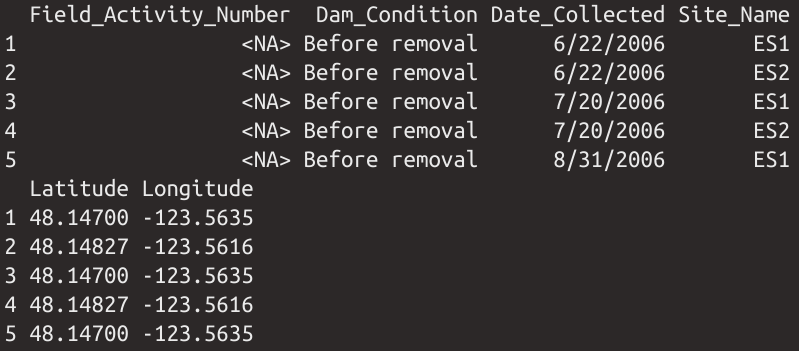
\includegraphics[scale=0.35]{images/a2-qst2.png}
    \end{center}

    {\color{gray}\item Provide the longitudinal and latitudinal coordinates for a Field-ID of your choice below. Make sure to include the Field-Activity-Number in your answer! \textbf{(1 pt)}}\par

    Field-ID 4: 48.14827 -123.5616
\end{enumerate}

\section*{Part 2: Descriptive Statistics}
\begin{enumerate}[font=\bfseries, wide, resume]
    {\color{gray}\item Walk through generating the descriptive statistics for pH values. Next, create similar R code to generate descriptive statistics (five-point summary) for both temperature and turbidity. Fill in the tables below and add descriptive table title descriptions to each. \textbf{(2 pts)}}\par

    \begin{table}[h]
        \centering
        \caption{Temperature (\SI{}{\celsius}) of water in the Elwha estuary from 2006 to 2014 \strut}
        \begin{tabular}{ccccc}
            \toprule
            Mean & Median & Minimum & Maximum & Stand Deviation \\
            \midrule
            13.11 & 12.35 & 5.79 & 20.98 & 3.29 \\
            \bottomrule
            \end{tabular}
    \end{table}

    \begin{table}[h]
        \centering
        \caption{Turbidity of water in the Elwha estuary from 2006 to 2014 \strut}
        \begin{tabular}{ccccc}
            \toprule
            Mean & Median & Minimum & Maximum & Stand Deviation \\
            \midrule
            63.23 & 13.9 & 0.3 & 305.6 & 88.98 \\
            \bottomrule
            \end{tabular}
    \end{table}
    {\color{gray}\item Calculate the 95\% confidence interval for temperature ($^\circ$C) and write a statement below including these values to assess our confidence in the temperature mean. \textbf{(2 pts)}}\par
    
    We have 95\% confidence that that the true mean temperature was between \SI{12.58}{\celsius} and \SI{13.65}{\celsius} assuming normal distribution.

\end{enumerate}

\section*{Part 3: Statistical Analyses in R}
\begin{enumerate}[font=\bfseries, wide, resume]
    {\color{gray}\item Walk through the t-test determining if the mean pH values are significantly different before and during dam removal. Next, determine if there is a significant difference in the mean turbidity values before and during dam removal by conducting your own t-test. Report your results in the context of the study by interpreting the p-value and variables used. \textbf{(2 pts)}}\par

    Turbidity was significantly higher during dam removal compared to before dam removal (t = -5.7058, df = 113.89, p-value = \SI{9.312e-08}).

    {\color{gray}\item Walk through the example ANOVA determining if the mean pH values are significantly different between different testing sites. Next, conduct your own ANOVA to determine if there are site differences in temperature during dam removal. Report your results in the context of the study by interpreting the p-value and variables used. \textbf{(2 pts)}}
    
    \begin{center}
        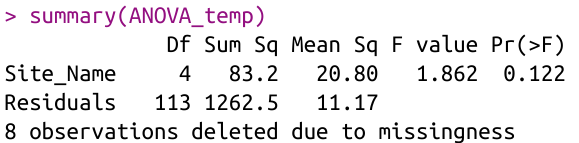
\includegraphics[scale=0.5]{images/a2-qst7.png}
    \end{center}

    There was no significant difference in temperature among sampling sites during dam removal (F=1.862; df=4,113; p=0.122).

    {\color{gray}\item Produce a boxplot to help illustrate your results from AQ-7. Export the image (copy to clipboard), paste below, and include a descriptive figure caption. \textbf{(2 pts)}}

    \begin{figure}[h]
        \centering
        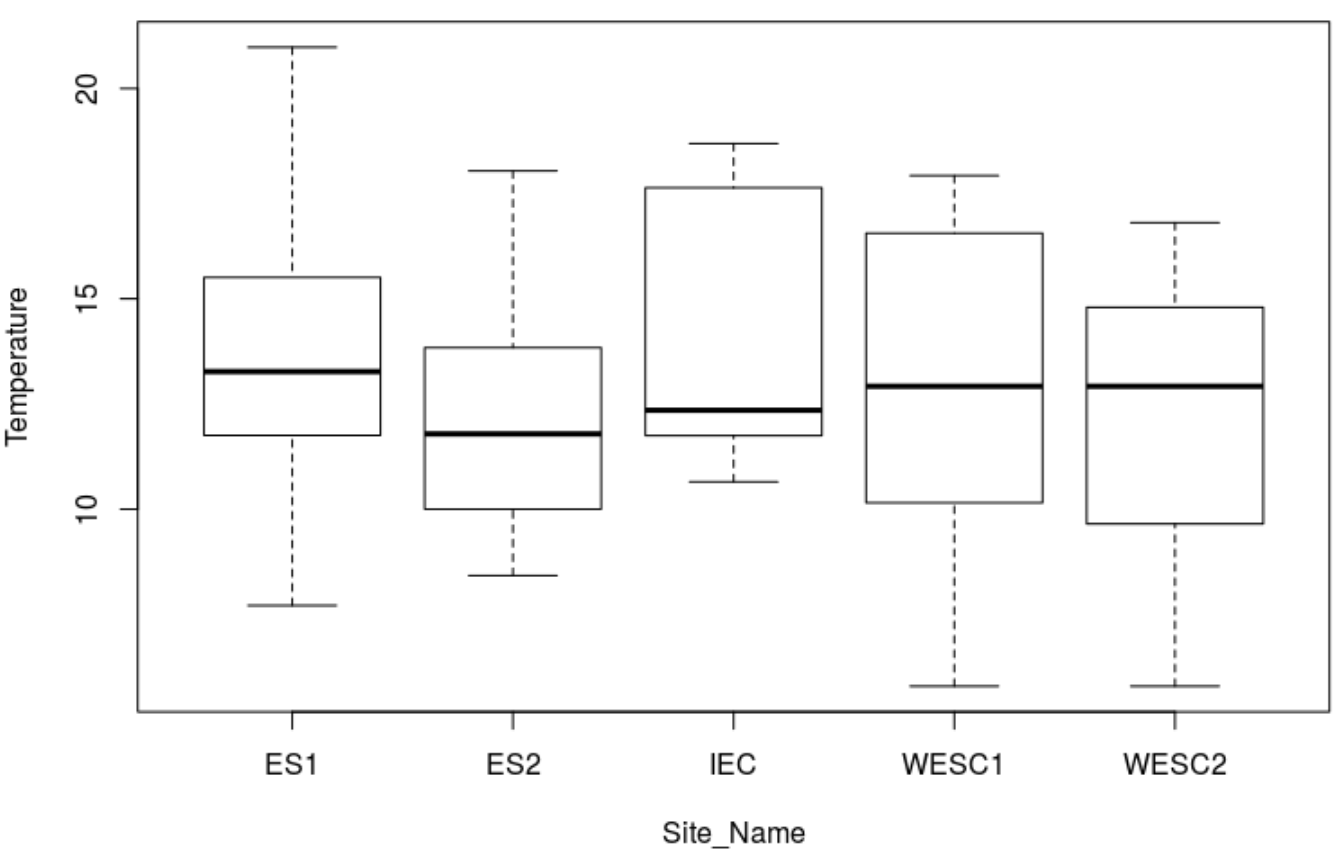
\includegraphics[scale=0.25]{images/qst8.png}
        \caption{Boxplot that shows outliers (the two open circles in ES1), medians (thick black lines in the middle of the boxes), quartiles (outer bounds of the boxes), and minimum and maximum values (excluding outliers; the lines at the end of the dotted-line arms) for turbidity before and after dam removal.}
        \label{}
    \end{figure}

    {\color{gray}\item What are the null hypotheses for each of the analyses (t-test; ANOVA) that you conducted above? \textbf{(1 pt)}}\par
    \begin{itemize}
        \item There is no significant difference turbidity before and after dam removal.
        \item There is no significant difference in temperature before and after dam removal. 
    \end{itemize}
\end{enumerate}

\section*{Part 4: Water quality}
\begin{enumerate}[font=\bfseries, wide, resume]
    {\color{gray}\item Why do you think dam removal would affect water quality parameters in a river? \textbf{(1 pt)}\par}

    Removal of the damn could change water flow which could introduce a wide range of effects, one being the water quality. 

    {\color{gray}\item What is turbidity? Why do you think it is an important parameter to consider when measuring water quality? Can you think of an example of very high turbidity? \textbf{(1 pt)}\par}

    Turbidity is how clear or transparent the water is. Higher turbidity means increased particles and lower visibility. Turbidity is important to consider because it lets you know how much of the water, isn't actually water. You want lower turbidity. An example of high turbidity would be a river during a flood, where there is an abnormally high amount of additional materiel flowing with the water. 

    {\color{gray}\item Why do you think water quality is important? Find an example from the primary literature to support your argument. What happens when there is poor water quality? What are some of the factors that contribute to poor water quality? \textbf{(2 pts)}\par}

    Water quality is important for a tremendous amount of reasons. From simple health, to crop yields, wildlife environments, and even proper control in scientific experiments. A good example from Grorud-Colvert and K. Sponaugle:

    \begin{quotation}
        ``Frequent loss of low settlement condition individuals and occasional loss of the very highest condition fish suggest that particularly high settlement condition during the warmest temperatures may be detrimental. Not only does the quality of settlers vary over time, but selective loss of individuals with particular phenotypic traits is not pervasive and can vary with environmental conditions such as temperature."
    \end{quotation}

    - Grorud-Colvert, K., Sponaugle, S. Variability in water temperature affects trait-mediated survival of a newly settled coral reef fish. Oecologia 165, 675–686 (2011). 

    {\color{gray}\item Think about a data-driven question that you would like to answer using RStudio. Find a potential dataset and describe it—what kind of variables it contains, what it measured, and what question you would like to use the data to answer. \textbf{(1 pt)}}\par

    I would love to analyze data received from grades in college, adjusted relative to peers (seriously the difference in teacher grading methods can be astounding), actual placement on tests like GRE and MCAT, combine it with highschool grades, related corse work done outside of school, family income, tragic events, and other such events then combine them to attempt to find the best predictors of success. 

    Perhaps I have not answered the correct question that this question is prompting, and I understand that the point is trying to get me to find real dataset to play with. But sadly, I have no idea where I would find such highly specified data sets for my question. I could change it, but I think I'll leave it as it is.  

    {\color{gray}\item What statistical test from the lab today would you use to analyze your data and why? What would be your null hypothesis? \textbf{(1 pt)}}\par

    I think other functions and means of modeling would be required to analyze the data set I would be interested in. Means of probability of outcome compared to real outcomes would be more desired, which would a combination of several tests. 

    I suppose my null hypothesis would be that single affect (grades, family, etc) DOES have an influence. I would expect no single event to give meaningful prediction.  
\end{enumerate}
\end{document}